\head{Апрель}{Листок 11. Делимость целых чисел -- 2.}

\section{Часть 3 -- "Евклидовая".}

\begin{center}
    \footnotesize{\textit{В задачах этого листка речь идёт только о целых числах.}}
\end{center}

\begin{center}
    \textit{\textbf{Лирическое отступление.}}
\end{center}

\begin{center}
  \fbox{\begin{varwidth}{0.95\textwidth}
      \begin{center}
          \textbf{Теорема Дирихле} \textit{(«о простых числах в арифметической прогрессии»)}
      \end{center}
    Каждое арифметическая прогрессия, первый член и разность которой -- натуральные, взаимно
    простые числа, содержит бесконечное число простых чисел.
    \end{varwidth}}  
\end{center}

Теорема Дирихле доказывается весьма сложно, и мы  в курсе её доказывать не будем. В 1950 году датский математик А. Сельберг придумал чрезвычайно сложное и хитроумное элементарное (не использующее аппарат высшей математики) доказательство теоремы Дирихле, однако жить лучше от этого не стало и даже сильно одарённому школьнику. Для желающих поломать голову добавим только, что по сути Дирихле доказал, что при любых фиксированных взаимно простых числах $m$ и $k$ $\underset{s \rightarrow 1+}{\textrm{lim}} \dfrac{ \underset{p}{\sum} \times \dfrac{1}{p^s}}{\textrm{ln} \frac{1}{s - 1}} = \dfrac{1}{\phi(k)}$, где суммирование ведётся по всем простым числам $p$ таким, что $p \equiv m~(\textrm{mod}~k)$, а $\phi (k)$ –- функция Эйлера. Это соотношение можно также интерпретировать как закон равномерного распределения простых чисел по классам вычетов по модулю $k$, так как при суммировании по всем простым числам $\underset{s \rightarrow 1+}{\textrm{lim}} \dfrac{ \underset{p}{\sum} \times \dfrac{1}{p^s}}{\textrm{ln} \frac{1}{s - 1}} = 1$. В качестве следствия из теоремы Дирихле можно также рассматривать утверждение, что ряд, составленный из обратных величин к простым числам из арифметической прогрессии, расходится. Красивым следствием из теоремы Дирихле является

\begin{center}
\fbox{\begin{varwidth}{0.95\textwidth}
    \begin{state}
        Не существует такого многочлена $f(x) = a_0 x^n + a_1 x^{n - 1} + ... + a_{n - 1}x + a_n$~с целыми коэффициентами такими, что все числа $f(0), f(1), f(2), f(3), ...$ являются простыми.
    \end{state}
    \end{varwidth}}
\end{center}

Впервые несложное доказательство этого факта придумал сам Эйлер. Он же напридумывал массу многочленов $f(x)$, значения которых при многих последовательных натуральных $x$ являются простыми числами. Например:

\begin{enumerate}[noitemsep, label=\asbuk*), ref=\asbuk*]
    \item $f(x) = x^2 + x + 41$, при $x = 0, 1, 2, ..., 39$.
    \item $f(x) = x^2 - 79x + 1601$, при $x = 0, 1, 2, ..., 79$.
\end{enumerate}

С первым многочленом вы должны быть хорошо знакомы -- мы рассматривали его в листке «Индукция», когда говорили о догадках по аналогии. Интересно, что если же рассматривать многочлены от нескольких переменных, то многочлены, множество положительных значений которых в точности является множеством всех простых чисел, существуют.\footnote{Этот факт был доказан Юрием Матиясевичем в 1970 году.} Нам удалось разыскать один из таких многочленов от 26 переменных, который и приводим здесь \smiley:

\begin{center}
$P(a, b, c, d, e, f, g, h, i, j, k, l, m, n, o, p, q, r, s, t, u, v, w, x, y, z) = \{k + 2\}\{1 - (wz + h + j – q)^2 - (2n + p + q + z – e)^2 – (a^2y^2 – y^2 + 1 – x^2)^2 – (\{e^4 + 2e^3\}\{a + 1\}^2 – o^2)^2 – (16\{k + 1\}^3\{k + 2\}\{n + 1\}^2 + 1 – f^2)^2 – (\{(a + u^4 – u^2a)^2 – 1\}\{n + 4dy\}^2 + 1 – \{x + cu\}^2)^2 – (ai + k + 1 – l – i)^2 – (\{gk + 2g + k + 1\}\{h + j\} + h – z)^2 – (16r^2y^4\{a^2 – 1\} + 1 - u^2)^2 – (p – m + l\{a – n – 1\} + b\{2an + 2a – n^2 – 2n – 2\})^2 – (z - pm + pla – p^2l + t\{2ap – p^2 – 1\})^2 – (q – x + y\{a – p – 1\} + s\{2ap + 2a – p^2 – 2p – 2\})^2 – (a^2l^2 – l^2 + 1 – m^2)^2 – (n + l + v – y)^2\}$
\end{center}

\section{Решение уравнений в целых числах.}

Отдельным большим разделом математики является область, посвящённая решению уравнений в целых числах. Эта математическая задача является одной из древнейших. Апогея своего расцвета эта область математики достигла в Древней Греции. Наиболее известным источником, дошедшим до нашего времени, является произведение Диофанта –- «Арифметика». Диофант суммировал и расширил накопленный до него опыт решения неопределённых уравнений в целых числах. И до сих пор целочисленные уравнения называются \textit{диофантовыми}.
\par
История сохранила нам мало черт биографии замечательного александрийского учёного-алгебраиста. По некоторым данным Диофант жил до 364 года н.э. Достоверно известно лишь своеобразное жизнеописание учёного, которое по преданию было высечено на его надгробии и представляло задачу-головоломку:

\textit{«Бог ниспослал ему быть мальчиком шестую часть жизни; добавив к сему двенадцатую часть, Он покрыл его щеки пушком; после седьмой части Он зажёг ему свет супружества и через пять лет после вступления в брак даровал ему сына. Увы! Несчастный поздний ребёнок, достигнув меры половины полной жизни отца, он был унесён безжалостным роком. Через четыре года, утешая постигшее его горе наукой о числах, он (Диофант) завершил свою жизнь» (попробуйте решить задачу самостоятельно).}

\begin{ex}
    Пусть $ax = by$ и НОД($a$, $b$) = 1. Докажите, что тогда найдётся такое число $t$, что $x = bt, y = at$.
\end{ex}

\begin{ex}
    Пусть $ax = by$ и НОД($a$, $b$) = 1. Опишите все пары целых чисел ($x$, $y$), являющиеся решениями данного уравнения.
\end{ex}

\begin{ex}
    Найдите все целые решения уравнения $12x + 14y = 0$.
\end{ex}

\begin{figure}[H]
\begin{minipage}{0.6\linewidth}
    Пусть на клетчатой бумаге нарисован прямоугольник размером $a \times b$ клеток (стороны прямоугольника идут по линии сетки). Проведём диагональ и отметим все узлы сетки, которые на ней лежат. На сколько частей эти узлы делят диагональ? (Узлами мы называем точки, где пересекаются линии сетки.)
    \begin{enumerate}[noitemsep, label=\asbuk*), ref=\asbuk*]
    \item  Решите задачу для прямоугольника размером 10$\times$15. (см. рис.)
    \item  Решите задачу в общем виде.
    \end{enumerate}
    \end{minipage}
    \hfill
\begin{minipage}{0.39\linewidth}
    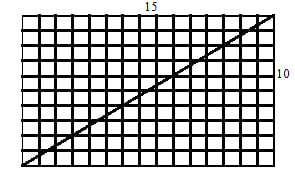
\includegraphics[width=0.95\columnwidth]{img/11.2 img1.jpg}
\end{minipage}
\end{figure}

Рассмотрим уравнение $ax + by = c$, где $a$, $b$ и $c$ -- целые числа. Наша задача -- определить, при каких условиях это уравнение имеет решение в целых числах $x$ и $y$, и какой вид имеют эти решения.

\begin{thm}
    Докажите, что уравнение $ax + by = c$ имеет решение в целых числах тогда и только тогда, когда $c$ делится на $d$ = НОД ($a$, $b$).
\end{thm}

\begin{thm}
    Докажите, что если НОД($a$, $b$) = 1, то уравнение $ax + by = c$ имеет бесконечное множество решений.
\end{thm}

\begin{thm} \ref{11.2 thm1}
    Докажите, что если пара чисел ($x_0$, $y_0$) -- решение уравнения $ax + by = c$, то все решения имеют вид $x = x_0 - bt$, $y = y_0 + at$, где $t$ -- любое целое число
\end{thm}

\textit{\underline{Замечание.}} Когда решение уравнения приводится в виде, зависящем от некоторого параметра, говорят, что приведено общее решение уравнения. Какое--нибудь конкретное значение чисел $x$ и $y$ называется частным решением исходного уравнения. Таким образом, ($x_0$, $y_0$) -- частное решение уравнения, а $x = x_0 - bt$, $y = y_0 + at$ -- общее решение исходного уравнения.

\begin{ex}
    Какие из приведённых ниже наборов чисел являются для уравнения $12x - 15y = 6$
    \par 
    1) решениями; 2) частными решениями; 3) общими решениями.
    \begin{enumerate}[noitemsep, label=\asbuk*), ref=\asbuk*]
        \item $x = -2$,~$y = -2$; 
        \item $x = 3 + 15t,~y = 2 + 12t$, где $t$ -- любое целое число;
        \item $x = -2 + 5t, y = -2 + 4t$, где $t$ -- любое
        целое число;
        \item $x = 15t, y = 12t$, где $t$ -- любое целое число; 
        \item $x = 3 + 5t, y = 2 + 4t$, где $t$ -- любое целое число.
    \end{enumerate}
\end{ex}

\begin{thm}
    Докажите, что если c делится на $d$ = НОД($a$, $b$) и $a$ = $a_1d$, $b = b_1d$, $c = c_1d$, то числа ($x_0$, $y_0$) одновременно являются или не являются решениями уравнений $ay - bx = c$ и $a_1y - b_1x = c_1$.
\end{thm}

\begin{thm}
    Имеют ли следующие уравнения решения в целых числах: 
    \par а) $6x - 16y = 220$; б) $105x + 42y = 56$?
\end{thm}

\begin{center}
    \textbf{Алгоритм Евклида.}\footnote{Евклид -- древнегреческий математик, автор первого из дошедших до нас теоретических трактатов по математике.}
\end{center}

\begin{figure}[H]
\begin{minipage}{0.15\linewidth}
    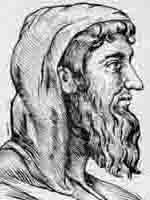
\includegraphics[width=0.95\columnwidth]{img/11.2 img2.jpg}
\end{minipage}
\hfill
\begin{minipage}{0.85\linewidth}
    Слово «алгоритм» означает «общий метод, применимый к целому классу задач». Обычно в математике подразумевается, что этот метод можно сформулировать в виде совершенно точного описания -- настолько точно и определенно, что любой человек, умеющий только читать и считать, может его выполнить (для любой конкретной задачи, т.е. для любых заданных ему значений параметров).
    \\
    \textit{Алгоритм Евклида} -- это правило, которое позволяет по двум натуральным числам $a$ и $b$ найти НОД($a$, $b$).
\end{minipage}
\end{figure}

Например, для нахождения наибольшего общего делителя двух чисел подходит и такой алгоритм:
\begin{enumerate}[noitemsep]
    \item найти все делители числа $a$ (перепробовать все числа: 1, 2, ..., не превосходящие $a$);
    \item найти все делители чисел $a$ и $b$ (проверив, на какие из делителей $a$ делится $b$);
    \item выбрать из общих делителей наибольший.
\end{enumerate}

\begin{figure}[H]
\begin{minipage}{0.74\linewidth}
    Конечно, если числа достаточно малы, то проще найти НОД, отыскав все делители обоих чисел или разложив оба числа на простые множители. А если числа очень велики и даже разложение на простые множители является проблематичным? Алгоритм Евклида позволяет найти НОД($a$, $b$) в этих случаях значительно быстрее, не отыскивая всех делителей ни у одного из чисел $a$ и $b$. Он основан на следующих фактах.
    \begin{thm}
        Докажите утверждение 4 из части 2, т.е. докажите, что НОД($b$, $a$ - $b$) = НОД($a$, $b$).
    \end{thm}
    \begin{thm}
        Пусть $a = bq + r$. Докажите, что тогда НОД($b$, $r$) = НОД($a$, $b$).
    \end{thm}
    Это утверждение позволяет легко и быстро находить НОД двух чисел.
    \\
    Покажем, как это делается.

% здесь нужно вставить таблицу
% \begin{table}[h]
% \begin{tabular}{ll}
%     $1014 = 2733 \times 3 + 195$ \hfill 
%     \\
%     $273 = 195 \times 1 + 78$ \hfill = 
%     \\
%     $195 = 78 \times 2 + 39$ \hfill = 
%     \\
%     $78 = 39 \times 2$ \hfill = 
%  & 
%      НОД(273, 1014) =
%     \\
%     НОД(195, 273) =
%     \\
%     НОД(195, 78) =
%     \\
%     НОД(78, 39) = 39
% \end{tabular}
% \end{table}
{
\begin{tabular}{ll}
$1014 = 2733 \times 3 + 195$ & НОД(273, 1014) = \\
$273 = 195 \times 1 + 78$ & = НОД(195, 273) = \\
$195 = 78 \times 2 + 39$ & = НОД(195, 78) = \\
$78 = 39 \times 2$ & = НОД(78, 39) = 39 \\
\end{tabular}
}

    \noindent \underline{Ответ:} НОД(273, 1014) = 39. \hfill \qedsymbol
\\
Приведённый выше метод отыскания наибольшего делителя и носит название \textit{алгоритма Евклида.}

Алгоритм Евклида в общем случае можно описать так: если имеются два целых числа $a$ и $b$, причем $a$ > $b$ > 0, то сначала делим $a$ на $b$, и получаем остаток $r_1$, который меньше, чем $b$. Затем делим число $b$ на $r_1$, находим остаток $r_2$, который меньше, чем $r_1$. Далее мы делим число $r_1$ на $r_2$, при этом получим остаток $r_3$, меньший, чем $r_2$ и так далее, пока какой-нибудь остаток $r_{n – 1}$ не разделится на остаток $r_n$ нацело, без остатка (т.е. $r_{n + 1} = 0$). Ясно, что указанный процесс обязательно кончится, поскольку каждый остаток меньше предыдущего, а все остатки -- неотрицательные числа. Последний остаток и есть НОД($a$, $b$). Действительно: 
\\
$r_n = НОД(r_n, r_{n - 1}) = НОД(r_{n - 1}, r_{n - 2}) = НОД(r_{n - 2}, r_{n - 3}) = ... = НОД(r_2, r_1) = НОД(r_1, b) = НОД(a, b)$.
\end{minipage}
\begin{minipage}{0.25\linewidth}
    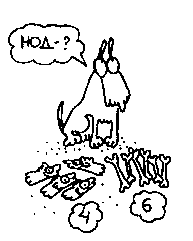
\includegraphics[width=0.95\columnwidth]{img/11.2 img3.png}
    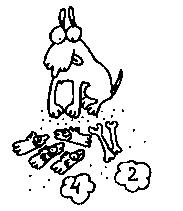
\includegraphics[width=0.95\columnwidth]{img/11.2 img4.png}
    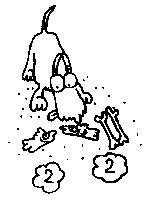
\includegraphics[width=0.95\columnwidth]{img/11.2 img5.png}
\end{minipage}
\end{figure}

\noindent \textbf{\textit{Пример.}} Найти НОД(273, 1014).

\textit{\textbf{Решение.}} Выполняем деление с остатком:
% \begin{figure}[H]
% \begin{minipage}{0.3\linewidth}
    % $1014 = 2733 \times 3 + 195$ \hfill 
    % \\
    % $273 = 195 \times 1 + 78$ \hfill = 
    % \\
    % $195 = 78 \times 2 + 39$ \hfill = 
    % \\
    % $78 = 39 \times 2$ \hfill = 
% \end{minipage}
% \begin{minipage}{0.3\linewidth}
    % НОД(273, 1014) =
    % \\
    % НОД(195, 273) =
    % \\
    % НОД(195, 78) =
    % \\
    % НОД(78, 39) = 39
% \end{minipage}
% \hfill
% \begin{minipage}{0.25\linewidth}
%     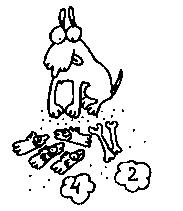
\includegraphics[width=0.95\columnwidth]{img/11.2 img4.png}
% \end{minipage}
% \end{figure}


\begin{ex}
    Найдите наибольший делитель чисел:
    \\
    а) 987654321 и 123456789; \hfill б) 16484 и 42282; \hfill в) 7777777777 и 777777.
\end{ex}

Покажем теперь, как алгоритм Евклида позволяет найти решение уравнения в целых числах. Согласно задаче \label{11.2 thm1} достаточно найти только какое--нибудь частное решение исходного уравнения, после чего общее решение тут же выписывается. Конечно, можно просто угадать, если же угадать сложно, то в нахождении такого решения как раз и поможет алгоритм Евклида. Если нужно решить уравнение $ax - by = c$ (можно считать, что $b$ > 0), отыскиваем с помощью алгоритма Евклида НОД($a$, $b$)

\begin{figure}[H]
    \centering
        \begin{minipage}{0.3\linewidth}
            $a = bq_0 + r_1;$
            \\
            $b = r_1q_1 + r_2;$
            \\
            $r_1 = r_2q_2 + r_3;$
            \\
            $...$
            \\
            $r_{n - 2} = r_{n - 1}q_{n - 1} + r_n;$
            \\
            $r_{n - 1} = r_nq_n$
        \end{minipage}
        \begin{minipage}{0.5\linewidth}
            $d = r_n$
            \\
            Теперь, возвращаясь по цепочке вверх, выписываем
            \\
            представление для $d$ через $a$ и $b$ в виде $a_{x_0} - b_{y_0}$.
            \\
            Найденные целые числа $x_0$ и $y_0$ и есть искомое
            \\
            частное решение исходного уравнения.
            \\

        \end{minipage}
\end{figure}

\begin{thm}
    Найдите решение уравнений в целых числах:
    \par а) 75y - 39x = 1; б) 43x + 250y = 7.
\end{thm}

\begin{thm}
    а) Костя живет в стандартном четырнадцатиэтажном доме в квартире 270. На каком этаже может располагаться его квартира? (На лестничной площадке одно и то же число квартир) 
    \par б)* Вообще, как быстро определить, может ли квартира с данным номером находиться на данном этаже?
\end{thm}

\begin{ques}
    Какая похожая задача была у нас в листке 5 про делимость?
\end{ques}